% mainfile: ../../main.tex
\chapter{Photoluminescence and excitons in semiconductors}\label{ch:exp:theory}
\AutoLettrine{Rats}
The effective masses of the holes along the growth-direction are
\begin{align}
    m_{\mr{hh},z}^{\ast} &= \frac{1}{\gamma_1 - 2\gamma_2} = 0.38 \\
    m_{\mr{lh},z}^{\ast} &= \frac{1}{\gamma_1 + 2\gamma_2} = 0.09
\end{align}
with
\begin{align}
    \gamma_1 &= 6.8 \\
    \gamma_2 &= 2.1.
\end{align}
In-plane, the masses then become
\begin{align}
    m_{\mr{hh},\parallel}^{\ast} &= \frac{1}{\gamma_1 + \gamma_2} = 0.11 \\
    m_{\mr{lh},\parallel}^{\ast} &= \frac{1}{\gamma_1 - \gamma_2} = 0.21
\end{align}

%Applying an out-of-plane electric field across the heterostructure pulls the electron and hole wavefunctions apart, resulting in a smaller overlap and at the same time a larger dipole moment.
%To assess the optical efficiency of a transition $m\to n$ under these two competing mechanisms, we can compute the oscillator strength~\cite{Davies2009}
%\begin{equation}\label{eq:exp:oscillator_strength}
%    f_{nm} = \frac{2\mu\Delta E_{nm}}{\hbar^2} \abs{\!\matrixelement{n}{z}{m}}^2,
%\end{equation}
%where $\Delta_{nm}$ is the transition energy.
%For the interband transitions of interest here, we use the reduced effective mass $\mu\inverse = m_{\mathrm{c}}\inverse + m_{\mathrm{hh}}\inverse$, and consider only transitions with $n=m$ as others are either not allowed or very weak.
%Finally, there is a certain gauge freedom in \cref{eq:exp:oscillator_strength} by choosing the origin of the coordinate system.
%For symmetry reasons, we choose the origin to be in the middle of the \gls{qw} and absorb the offset into a constant term, $f_{nm}\rightarrow f_{nm}\gth{0} + \Delta f_{nm}$, where only the latter term depends on the electric field.
% the actual transition matrix element is in-plane. but the wave function does not change in-plane, so only the reduced overlap contributes.

\clearpage

\begin{marginfigure}
    \centering
    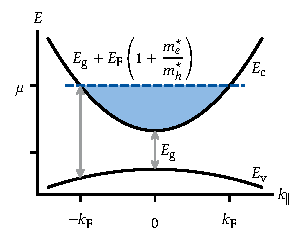
\includegraphics{img/pdf/experiment/2deg_sketch}
    \caption[\imgsource{img/py/experiment/pl.py}]{
        Band structure diagram of a doped heterostructure (after \citer{Kamburov2017}).
        Due to the $n$-type doping, the conduction band is filled up to the Fermi level $\mu$.
        Photonic excitation of an electron-hole pair can only occur at $\abs{k} > k_\mr{F}$ into the free states above $\mu$ due to the small photon momentum.
        Recombination can occur within a bandwidth of $E_\mr{F}(1 + m^\ast_{\mr{c}}/m^\ast_{\mr{hh}})$.
    }
    \label{fig:exp:theory:bandstructure}
\end{marginfigure}

\begin{marginfigure}
    \centering
    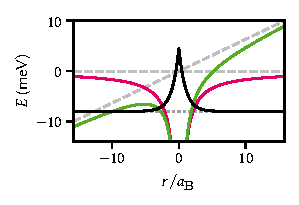
\includegraphics{img/pdf/experiment/in_plane_field}
    \caption[\imgsource{img/py/experiment/qcse.py}]{
        Effect of an in-plane electric field on an exciton wavefunction.
        In the hole's reference frame, the electron sees a static attractive Coulomb potential (magenta), resulting in a bound state (dotted gray line, wave function sketched in black).
        Applying an electric field ($F=\qty{100}{\milli\volt\per\micro\meter}$, dashed gray lines) tilts the Coulomb potential (green) and leads to a transparent barrier through which the electron can tunnel out.
    % In-plane fields -> field ionization -> line broadening \cite{Miller1985}
    }
    \label{fig:exp:theory:in_plane_field}
\end{marginfigure}

\clearpage

\section{The \acrlong{qcse}}\label{sec:exp:theory:qcse}
In order to obtain a qualitative understanding of the influence of an electric field on the \gls{pl}, consider an undoped \ch{GaAs/Al_{0.33}Ga_{0.66}As} \gls{qw} of width $L = \qty{20}{\nano\meter}$.
We take a 57:43 ratio for the band offsets~\cite{Miller1984a}, resulting in discontinuities of height $\Delta E_{\mr{c}} = \qty{0.24}{\electronvolt}$ and $\Delta E_{\mr{hh}} = \qty{0.18}{\electronvolt}$ at the interfaces for the conduction and the heavy-hole valence band, respectively, and $m^\ast_{\mr{c}}/m_e = \num{0.067}$ and $m^\ast_{\mr{hh}}/m_e = \num{0.34}$ for the effective masses.\sidenote{
    I note that the literature knows many different values for the hole effective mass in the plane of a quantum well, suggesting that one should actually measure it to be confident in the actual value.
}
Assuming an infinitely deep well for simplicity, the eigenenergies are
\begin{equation}\label{eq:exp:theory:square_well:eps}
    E_n = \frac{1}{2 m^\ast}\left[\frac{\pi\hbar n}{L}\right]^2
\end{equation}
and the eigenstates are
\begin{equation}\label{eq:exp:theory:square_well:psi}
    \psi_n(z) = \sqrt{\frac{2}{L}}\sin(\frac{n\pi z}{L}).
\end{equation}
The ground state energy is then \qty{14}{\milli\electronvolt} (\qty{3}{\milli\electronvolt}) above the band edge, corresponding to \qty{6}{\percent} (\qty{2}{\percent}) of the respective band offsets and implying that the infinite-well approximation is acceptable.\sidenote{
    In a finite well, the wavefunctions decay exponentially into the barriers and result in slightly lower eigenenergies.
    However, the qualitative behavior remains the same.
}
The upper panel of \cref{fig:exp:theory:bandstructure} depicts the first two wavefunctions of electrons and holes in a band structure diagram.
Due to the symmetry of the confining potential, the wavefunctions are symmetric around the center of the well.

\begin{marginfigure}
    \centering
    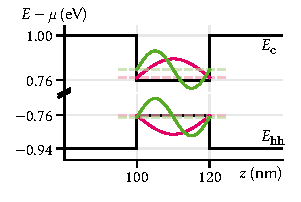
\includegraphics{img/pdf/experiment/qw_undoped_0V}
    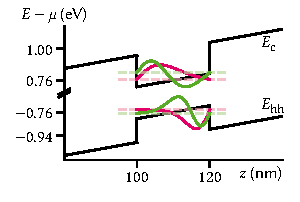
\includegraphics{img/pdf/experiment/qw_undoped_1V}
    \caption[\imgsource{img/py/experiment/qcse.py}]{
        \Gls{qcse} in an undoped \acrshort{qw}.
        Top: conduction and heavy-hole valence band profiles along the growth direction.
        The wavefunctions of the first two eigenstates in the well are drawn in magenta and green, respectively.
        The ground state transition is larger by $\Delta E = \qty{17}{\milli\electronvolt}$ than the gap $E_{\mr{g}}$ due to the confinement.
        Bottom: same structure as above with an out-of-plane electric field applied across the structure ($F=\qty{5}{\volt\per\micro\meter}$).
        Analytical wavefunctions in the infinite-well approximation are shown in magenta and green again.
        The wavefunctions get pushed to opposite interfaces of the \acrshort{qw}, lowering the ground state transition energy by $\Delta E = -\qty{10}{\milli\electronvolt}$.
        Excitonic effects are not included.
    }
    \label{fig:exp:theory:qw_tilted}
\end{marginfigure}

Now, applying an out-of-plane electric field tilts the bands and pulls electrons and holes to opposite interfaces of the \gls{qw}.
The Hamiltonian for the electrons in this case reads~\cite{Rabinovitch1971,Miller1985,Davies2009}
\begin{equation}\label{eq:exp:theory:qcse:hamiltonian}
    H = -\frac{\hbar^2}{2m^\ast}\dv[2]{z} + eFz
\end{equation}
if we take $z$ to be zero at an interface and choose $F \geq 0$.
Introducing the length and energy scales~\cite{Davies2009}
\begin{align}
    \tilde{\eps} &= \left[\frac{\left(\hbar eF\right)^2}{2m^\ast}\right]^{\frac{1}{3}}, \\
    \tilde{z} &= \left[\frac{\hbar^2}{2m^\ast eF}\right]^{\frac{1}{3}} = \frac{\tilde{\eps}}{eF},
\end{align}
and defining
\begin{equation}
    Z_n = z/\tilde{z} - \eps_n/\tilde{\eps}
\end{equation}
with $\eps_n$ the eigenenergy, the Schrödinger equation becomes~\cite{Rabinovitch1971}
\begin{equation}\label{eq:exp:theory:qcse:se}
    \dv[2]{Z_n}\psi_n(Z_n) = Z_n\psi_n(Z_n).
\end{equation}
\Cref{eq:exp:theory:qcse:se} is known as the Stokes or Airy equation and has the general solution
\begin{equation}
    \psi_n(Z_n) = \alpha_n\Ai(Z_n) + \beta_n\Bi(Z_n),
\end{equation}
where $\Ai(z)$ and $\Bi(z)$ are the Airy functions.
The $\Ai(z)$ and $\Bi(z)$ oscillate for $z < 0$ and decay (grow) exponentially for $z > 0$, respectively.
As we assumed infinitely high barriers at $z = 0$ and $z = L$, the boundary conditions impose
\begin{equation}
    \psi_n(0) = \psi_n(L) = 0,
\end{equation}
which completely determines the eigenstates and -energies.
For large well widths or fields ($eFL/\eps_n\gg 1$), the second term is exponentially suppressed and the eigenenergies are given by the zeros of $\Ai(Z_n)$.
For zero field, one recovers the square well solution (\cref{eq:exp:theory:square_well:psi,eq:exp:theory:square_well:eps}).

The finite-field case is shown in the lower panel of \cref{fig:exp:theory:bandstructure} for $F=\qty{5}{\volt\per\micro\meter}$.
Due to the larger effective mass of the heavy holes, the characteristic length scale $\tilde{z}$ is shorter and hence the corresponding wavefunctions are narrower than their electronic counterparts.
The ground state transition energy at this field is \qty{10}{\milli\electronvolt} below the gap or \qty{27}{\milli\electronvolt} lower than in the zero-field case.

For a full quantitative accounting of the transition energies, the exciton binding energy as well as finite barrier heights would be required.
The former is on the order of \qtyrange{6}{9}{\milli\electronvolt} in \ch{GaAs} and becomes smaller as the overlap of the electron and hole wavefunctions is reduced when applying an electric field, pulling the wavefunctions to opposite interfaces.
\Citet{Miller1985} found that finite-well properties could be reproduced by using effective well widths with infinite well models.

The latter should have a small effect on the ground state energy as argued above.
Additionally, tilting the \gls{qw} results in a finite probability for the charge carriers confined within the well to escape as -- for infinitely thick barriers -- lower-lying states become available at some distance away, an effect known as Fowler-Nordheim tunneling.
%This naturally also leads to a loss in radiative recombination efficiency.
Following \citer{Davies2009}, we can estimate the tunneling probability as
\begin{equation}
    \mathscr{T}_n(F) \approx \exp\left\lbrace -\frac{\sqrt{4 m^\ast (\Delta E_{\mr{c}(\mr{hh})} - \eps_n)^3}}{e F\hbar}\right\rbrace,
\end{equation}
where $\Delta E_{\mr{c}(\mr{hh})}$ is the conduction (valence) band offset.
% TODO: move to figure?

\subsection{In-plane confinement}\label{subsec:exp:theory:qcse:trap}
% Motivate why we do all this! -> oscillator strength
So far, we have considered the \gls{qcse} in a single dimension, as if we were to apply a global electric field.
However, as we saw before, the field lowers the exciton energy below the \gls{qw} confinement and hence, if applied locally, results in an effective confinement potential in the plane of the \gls{qw}.
\citet{Descamps2021} performed numerical simulations for a geometry with circular gate electrodes with \qty{200}{\nano\meter} diameter on both sides of a membrane, finding a confinement depth of \qty{20}{\milli\electronvolt} at $F=\qty{5}{\volt\per\micro\meter}$ that is well approximated by a single-particle harmonic potential with confinement strength $\omega/2\pi = \qty{738}{\giga\hertz}$ corresponding to an oscillator length $\xi=\sqrt{\hbar/M\omega}=\qty{20}{\nano\meter}$.

How does this in-plane confinement modify the wavefunction?
The harmonic potential applies to the center-of-mass wavefunction of the exciton with mass $M = m^\ast_{\mr{c}} + m^\ast_{\mr{hh}}$.
We ignore the relative motion of electron and hole as the optical properties of the exciton are dominated by the behavior at zero separation for $a_{\mr{B}}/\xi < 1$~\cite{Kavokin1994}, where $a_{\mr{B}}=2\pi\eps_0\eps_{\mr{r}}\hbar^2/\mu e^2=\qty{6}{\nano\meter}$ is the exciton Bohr radius in two dimensions with $\epsilon_{\mr{r}} = \num{13.3}$ in \ch{GaAs} at low temperatures and $\mu$ the reduced effective mass~\cite{Olsen2016}, and consider only $\Delta n = 0$ transitions, \ie, electron and hole in the same $z$ quantum state, as $\Delta n\neq 0$ transitions are much weaker~\cite{Davies2009}.
Let us further initially assume a separable wavefunction and choose cylindrical coordinates according to the symmetry of the potential.
We then have
\begin{equation}\label{eq:exp:theory:qcse:trap:psi}
    \Psi_{np\ell}(z_e, z_h, \rho, \phi) = \psi_n(z_e)\psi_n(z_h)\chi_{p\ell}(\rho)\exp(i\ell\phi)
\end{equation}
where~\cite{Karimi2014}\sidenote{
    Note that \citeauthor{Karimi2014} miss a factor $2\pi$ in the normalization.
}
\begin{equation}\label{eq:exp:theory:qcse:trap:ho:psi}
    \chi_{p\ell}(\rho, \phi) = \sqrt{\frac{2p!}{2\pi\xi^2(p + \abs{\ell})!}}\exp(-\tilde{\rho}^2/2)\tilde{\rho}^{\abs{\ell}}L_p^{\abs{\ell}}\left(\tilde{\rho}\right)
\end{equation}
with the associated Laguerre polynomial $L_p^{\abs{\ell}}(x)$ and we used the shorthand $\tilde{\rho} = \rho/\xi$.
The numbers $p\in\mathbb{N}$ and $\ell\in\mathbb{Z}$ denote the principal and orbital momentum quantum numbers.
The eigenenergies of the harmonic oscillator solution \cref{eq:exp:theory:qcse:trap:ho:psi} are given by
\begin{equation}\label{eq:exp:theory:qcse:trap:ho:eps}
    \eps_{p\ell} = \hbar\omega\left(2p + \abs{\ell} + 1\right).
\end{equation}
To account for a finite well width ($L\approx\xi$ in our case), we can to a first approximation perform the replacement $\rho\to r = \sqrt{\rho^2 + z^2}$ in \cref{eq:exp:theory:qcse:trap:psi}.
The resulting wavefunction $\Psi_{np\ell}(r, z_{\mr{h}})$ at fixed electron coordinate $z_{\mr{e}}$ is shown in \cref{fig:exp:theory:qcse:wf} for $n = \ell = 0$ (which makes it independent of $\phi$).

At last, we can use the exciton wavefunction $\Psi_{nm\ell}(r, \phi, z_{\mr{e}}, z_{\mr{h}})$ to estimate the \emph{oscillator strength}, a quantity often quoted in semiconductor spectroscopy.
The oscillator strength puts in relation the quantum mechanical transition rate with the emission rate of a classical oscillator with frequency $\omega = \Delta E/\hbar$~\cite{Hilborn1982}.
For a dipole transition from state $\ket{i}$ to state $\ket{j}$, it may be written as~\cite{Davies2009}
\begin{equation}\label{eq:exp:oscillator_strength}
    f_{ji} = \frac{2\mu\Delta E_{ji}}{\hbar^2} \abs{\!\matrixelement{j}{\bvec{r}}{i}}^2,
\end{equation}
where $\mu$ is the reduced mass of the exciton.
As the selection rules only allow in-plane dipole transitions for heavy holes, we write~\cite{Kavokin1994}
\begin{equation}
    f_{np\ell} = \frac{2\mu\Delta E_{np\ell}}{\hbar^2} J_{r}^2 J_{\phi}^2 \abs{\!\matrixelement*{u_{\mr{c}}}{x}{u_{\mr{hh}}}}^2
\end{equation}
for transitions with $\Delta n = \Delta p = \Delta\ell = 0$, where
\begin{align}
    J_{r} &= \int_{0}^{L}\dd{z}\int_0^{\infty}\dd{\rho}\rho\psi_n\gth{\mr{e}}(z)\psi_n\gth{\mr{h}}(z)\chi_{p\ell}(\sqrt{\rho^2 + z^2}), \\
    J_{\phi} &= \int_0^{2\pi}\dd{\phi}\exp(\i\ell\phi),
\end{align}
and $\ket*{u_{\mr{c}(\mr{hh})}}$ are the Bloch functions of the valence and conduction band, respectively, that we have neglected so far.

$\ell\neq 0$, $\Delta\eps_{p\ell} = 2p = \qty{1}{\milli\electronvolt}$ (\cf~\citer{Descamps2021})


\begin{figure}
    \centering
    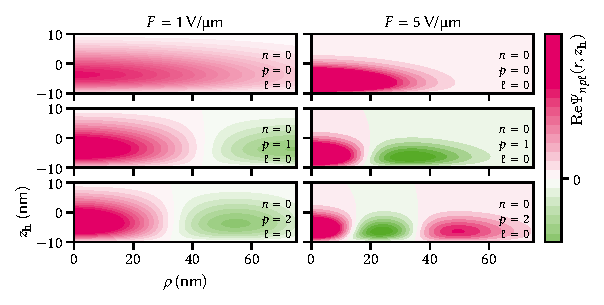
\includegraphics{img/pdf/experiment/wavefunction}
    \caption[\imgsource{img/py/experiment/qcse.py}]{
        Center-of-mass exciton wavefunction (hole sector) in a harmonic trap under an electric field.
        Left column shows the zero-field and right column the high-field case.
        Top row is the ground state and bottom row the first excited state in the plane.
        The out-of-plane wavefunction is the ground state in all cases ($n=0$) and the trap confinement strength $\omega/2\pi = \qty{738}{\giga\hertz}$~\cite[Sec.~2.2.2]{Descamps2021}.
    }
    \label{fig:exp:theory:qcse:wf}
\end{figure}


\begin{marginfigure}
    \centering
    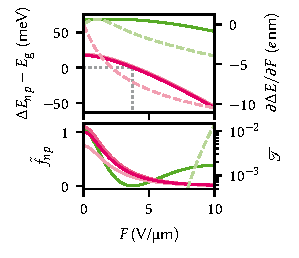
\includegraphics{img/pdf/experiment/qcse_field_dependence}
    \caption[\imgsource{img/py/experiment/qcse.py}]{
        Electric field dependence of the \gls{qcse} for the first two energy levels in the \gls{qw}.
        Top: the ground state energy (magenta) shows the expected quadratic dependence; the confinement energy is compensated at around $F=\qty{3.7}{\volt\per\micro\meter}$.
        Dashed lines (right axis) show the derivative, revealing that the excited state is actually raised in energy at low fields.
        Bottom: oscillator strengths (same color code as above).
        Despite the fact that the wavefunctions are pulled apart by the electric field, the oscillator strength of the ground state has a maximum at around \qty{2.5}{\volt\per\micro\meter}.
        Dashed lines (right axis) show the tunneling probability through the barrier.
        Only the excited electron state is appreciably non-zero at large fields.
    }
    \label{fig:exp:theory:qcse:field}
\end{marginfigure}

